\newpage
\section{Example: Minesweeper}
In this section, we will develop a simple implementation of the well-known {\em Minesweeper} game.  Typically the minesweeper game is played through a graphical user interface, illustrated as follows:
\begin{center}
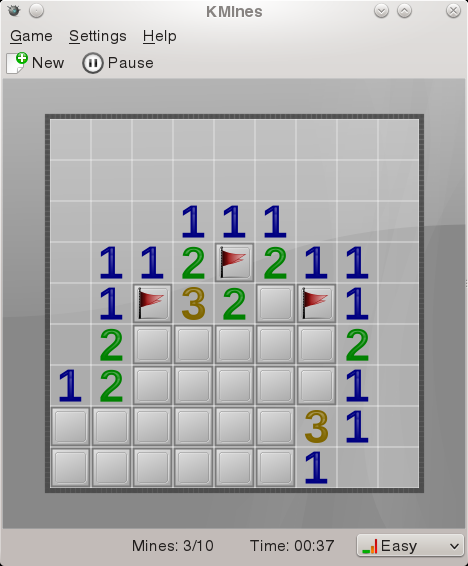
\includegraphics[width=0.35\textwidth]{../images/kmines.png}
\end{center}
Here, we can see the main aspects of the game.  The {\em game board} is a two-dimensional grid of {\em squares}.  Each square holds {\em nothing} or a {\em bomb} and is in one of the three states: {\em hidden}, {\em exposed} or {\em flagged} (with a flag).  An exposed square shows either the total number of bombs in the nine adjacent squares, referred to as its {\em rank}.  If an exposed square contains a bomb, then the game is over and the player has lost.  Flagged squares are protected and cannot be exposed unless they are {\em unflagged}.  The intuition here, is that the player marks those squares believed to contain a bomb.  

Let's analyse the above board.  In the following diagram of the above minesweeper game, gray squares represent hidden squares in the game.  For our benefit here, we've split them into two categories: those which contain a bomb (dark gray); and, those which don't: 

\begin{center}
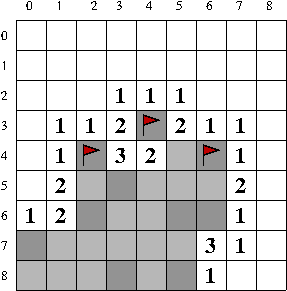
\includegraphics[width=0.35\textwidth]{../images/kmines_analysis.png}
\end{center}

In our discussion, we'll use $(x,y)$ to indicate a position on the board where $x$ gives the horizontal component, and $y$ the vertical component.  So, for example, the squares $(2,4)$, $(4,3)$ and $(6,4)$ are all marked with a flag.  Indeed, we can see that the above player has correctly flagged the three bombs in these squares, and that there are seven remaining to be identified and flagged.  Of course, unlike us, the player cannot see exactly where the bombs are.  However, he/she can easily determine that the square $(2,6)$ must contain a bomb.  This is because the exposed square at $(1,4)$ has a rank of $1$, and a bomb is flagged at $(2,4)$.  Therefore, there can be no bomb in square $(2,5)$ as this mean the rank of square $(1,4)$ was incorrect.  Finally, the rank of the square at $(1,5)$ is $2$ with only three unexposed squares, of which one is known already to contain a bomb and the other is known {\em not} to contain a bomb.  Therefore, the $(2,6)$ must contain a bomb.

The player plays the game by repeatedly selecting a square to expose.  When all squares are exposed, except for those containing bombs, the game is over and the player wins.  However, if a square holding a bomb is exposed, then the game is over immediately and the player loses.  A {\em blank} square is one with no adjacent bombs.  When a blank square is exposed, every adjacent blank square is recursively exposed.

\subsection{Squares}
We're now going to begin implementing the game of Minesweeper in Whiley.  To start with, we'll implement the game board in Whiley and provide functions for manipulating it; then, we'll implement the gameplay itself.  

The first aspect of the game board we'll implement is the concept of a {\em square}.  There are essentially two broad categories of square in the game: {\em exposed squares} and {\em hidden squares}.  Therefore, our implementation will reflect this.  Exposed squares either have a {\em rank} or are {\em blank} (i.e. have a rank of zero).  Furthermore, they may or may not hold a bomb.  We can implement this in Whiley like so:
\begin{lstlisting}
type ExposedSquare is { 
  int rank,       // Number of bombs in adjacent squares
  bool holdsBomb  // true if the square holds a bomb
}
\end{lstlisting}
Here, we can see that an integer field called \lstinline{rank} is used to store the rank of the square.  Likewise, a boolean field called \lstinline{holdsBomb} is used to indicate whether or not the square holds a bomb.  To simply creating values of type \lstinline{ExposedSquare}, it is common to additionally provide one or more {\em constructors}.  These are functions of the same name which create values of the given type.  Here is our \lstinline{ExposedSquare} constructor:

\begin{lstlisting}
// ExposedSquare constructor
function ExposedSquare(int rank, bool bomb) => ExposedSquare:
    return { rank: rank, holdsBomb: bomb }
\end{lstlisting}


Hidden squares may or may not hold a bomb, and may or may not have been flagged.  We can implement this in Whiley as follows:

\begin{lstlisting}
type HiddenSquare is { 
  bool holdsBomb,  // true if the square holds a bomb
  bool flagged     // true if the square is flagged
}

function HiddenSquare(bool bomb, bool flag) => HiddenSquare:
    return { holdsBomb: bomb, flagged: flag }
\end{lstlisting}

As before, a boolean field called \lstinline{holdsBomb} is used to signal whether or not the square holds a bomb.  Likewise, a boolean field called \lstinline{flagged} signals whether or not the square is flagged.  

We can now define the concept of a square in our Whiley implementation by combining the notions of exposed and hidden squares together as follows:

\begin{lstlisting}
type Square is ExposedSquare | HiddenSquare
\end{lstlisting}

Here, the type \lstinline{Square} is a union of the types \lstinline{ExposedSquare} and \lstinline{HiddenSquare}.  In otherwords, it is either an \lstinline{ExposedSquare} or a \lstinline{HiddenSquare}.  Notice that we don't provide a constructor for \lstinline{Square}.  This is because a \lstinline{Square} is merely the composition of two existing types with their own constructors.

\subsection{Board}

Using our above \lstinline{Square} data type, we can now define the game board in our Whiley implementation as follows:

\begin{lstlisting}
type Board is {
   [Square] squares,  // List of squares making up the board
   int width,         // Width of the game board (in squares)
   int height        // Height of the game board (in squares)
}
\end{lstlisting}

The main component of \lstinline{Board} is the \lstinline{squares} list.  Although this is a one-dimensional list, we'll see shortly that it is treated a two dimensional way.  The remaining fields record the width and height of the board, which is needed in order to safely manipulate the board.  To accompany this data type, we define a simple constructor as follows:
\begin{lstlisting}
// Create a board of given dimensions which contains no bombs, and
// where all squares are hidden.
Board Board(int width, int height):
    [Square] squares = []
    //
    for i in 0 .. width * height:
      squares = squares ++ [HiddenSquare(false,false)]
    //
    return {
        squares: squares,
        width: width,
        height: height
    }
\end{lstlisting}
This constructor creates a \lstinline{Board} of given width and height containing only hidden squares and no bombs.  Later, we will return to consider how to randomly place bombs on the board..

We will return to define a constructor for \lstinline{Board} shortly, but first we will provide some simpler helper functions for updating the board.  First, we provide a function to read the \lstinline{Square} at a given position on a \lstinline{Board}:

\begin{lstlisting}
// Return the square on a given board at a given position
function getSquare(Board b, int col, int row) => Square:
    int rowOffset = b.width * row // calculate start of row
    return b.squares[rowOffset + col]
\end{lstlisting}

This function performs a simple calculation to determine the start of the row in the \lstinline{Board.squares} list.  To understand this calculation, we need to view the board in a 1-Dimensional manner, as follows:

\begin{center}
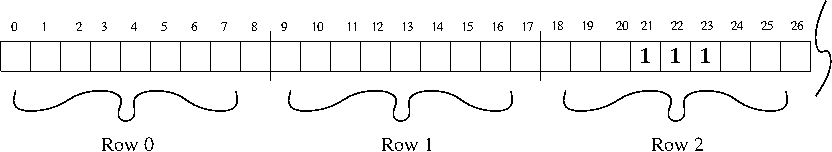
\includegraphics[width=0.95\textwidth]{../images/kmines_flat.png}
\end{center}

Here, we can see how each row is laid out in the 1-Dimensional list \lstinline{Board.squares}.  To calculate the start of a given row, we multiple the row number by the width of the board.  Then, to calculate a given column within that row, we simply add the column number.  For example, the position $(3,2)$ represents column 2, row 3; therefore, the position in the example board above would be: $(2 * 9) + 3 = 21$.

The corresponding function to the above provides a way to change the square at a given position on the board:

\begin{lstlisting}
// Set the square on a given board at a given position
function setSquare(Board b, int col, int row, Square sq) => Board:
    int rowOffset = b.width * row // calculate start of row
    b.squares[rowOffset + col] = sq
    return b
\end{lstlisting}

Here, the same calculation is performed as before to determine the actual position within the \lstinline{Board.squares} list.  This time, the \lstinline{Board.squares} array is updated with the new \lstinline{Square}.  Note that we must return the updated board in order for this change to be visible (see~\ref{value_semantics} for more on this).  Notice also that we are not attempting to control how the \lstinline{Board.squares} list may be updated.  That is, any \lstinline{Square} can be passed into this function, even it doesn't make sense in the wider context of the game.  These provide some general-purpose mechanisms for manipulating a \lstinline{Board}.

\subsection{Game Play}

Having defined the data types for the Minesweeper game, we can use these to implement the actions of the game.  In particular, the user can {\em flag squares} and {\em expose squares}.  We also need to know when its {\em game over} and the player has either {\em won} or {\em lost}.  The easiest of these is that for flagging squares:

\begin{lstlisting}
// Flag (or unflag) a given square on the board.  If this operation is not permitted, then do nothing
// and return the board; otherwise, update the board accordingly.
function flagSquare(Board b, int col, int row) => Board:
   Square sq = getSquare(b,col,row)
   // check whether permitted to flag
   if sq is HiddenSquare:
      // yes, is permitted so reverse flag status and update board
      sq.flagged = !sq.flagged
      b = setSquare(b,col,row,sq)
   //
   return b
\end{lstlisting}

This function checks whether the square on the board is hidden or not.  If so, the flagged status of that square is flipped (i.e. if it was not flagged then it is now, etc).  As before,  we must return the updated board in order for any change to be visible (see~\ref{value_semantics} for more on this).

The next function we'll implement is that for exposing a square.  This requires that the square to be exposed is not already exposed.  Furthermore, in the case of a blank square, then the expose method is recursively applied to blank squares.  An important sub-computation to this process is that of determining the rank of a given square.  That is the number of bombs contained in adjacent squares.  Here is our implementation of this sub-function:

\begin{lstlisting}
int determineRank(Board b, int col, int row):
    int rank = 0
    for r in (row-1) .. (row+2):
        for c in (col-1) .. (col+2):
            Square sq = getSquare(b,c,r)
            if sq.holdsBomb:
                rank = rank + 1
    //
    return rank
\end{lstlisting}

This function iterates through the nine squares which directly surrounding that specified by \lstinline{col} and \lstinline{row}.  Note that the range \lstinline{col-1 .. col+2} returns the three values \lstinline{col-1}, \lstinline{col} and \lstinline{col+1} (i.e. up to but not including \lstinline{col+2}).  Also, note that we can access the field \lstinline{holdsBomb} without determining whether \lstinline{sq} is hidden or not.  This is because \lstinline{holdsBomb} is contained in both \lstinline{ExposedSquare} and \lstinline{HiddenSquare} and, hence, is guaranteed to be present for any \lstinline{Square}.

Using the \lstinline{determineRank()} function above, we can now specify the following function for exposing a given square on the board:

\begin{lstlisting}
// Attempt to recursively expose blank hidden square, starting from a given position.
function exposeSquare(Board b, int col, int row) => Board:
   // first, ensure square to expose is valid
   if col < 0 || row < 0 || col >= b.width || row >= b.height:
       return
   // second, check whether is blank hidden square
   Square sq = getSquare(b,col,row)
   int rank = determineRank(b,col,row)
   if sq is HiddenSquare:       
      // yes, so expose square
      sq = ExposedSquare(rank,sq.holdsBomb)
      b = setSquare(b,col,row,sq)
      if rank == 0:
          // now expose neighbours
          for r in (row-1) .. (row+2):
              for c in (col-1) .. (col+2):
                  b = exposeSquare(b,c,r)
   //
   return b
\end{lstlisting}

This function does one of two things depending on the square being exposed.  First, the square is exposed by by creating an \lstinline{ExposedSquare} and updating the board.  Then, if that square is blank (i.e. has a rank of zero), then it and its neighbours are recursively exposed by calling \lstinline{exposeSquare()} again.

The final function we need to implement the game is that for determining when the game is actually over and, furthermore, whether the player has won or not.  This examines the board to see whether there are any exposed squares (in which case, the game is over and the player lost).  Furthermore, it checks whether or not every hidden squares contains a bomb (in which case, the game is over and the player won).  This function is implemented as follows:

\begin{lstlisting}
function isGameOver(Board b) => (bool,bool):
    bool isOver = true
    bool hasWon = true
    for i in 0 .. |b.squares|:
        Square sq = b.squares[i]
        if sq is HiddenSquare && !sq.holdsBomb:
            // Hidden square which doesn't hold a bomb so game may not be over
            isOver = false
        else if sq is ExposedSquare && sq.holdsBomb:
            // Exposed square which holds a bomb so game definitely over
            isOver = true
            hasWon = false
            break
    //
    return isOver, hasWon
\end{lstlisting}
This function iterates through every square on the board, and checks for two cases: firstly, whether a hidden square exists which does not contain a bomb; secondly, whether there is an exposed bomb.  Note that, if an exposed bomb is found the loop exits immediately; however, if a hidden square is found which doesn't hold a bomb we must continue to examine the remaining squares to see whether an exposed bomb exists or not.